\chapter{绪论}\label{ch:intro}

随着人工智能概念的兴起和增强现实(Augment Reality,以下简称AR)、无人机、移动机器人、自动驾驶等行业的发展,工业界与学术界对高精度、高效率、高鲁棒性的三维感知的需求越来越大。这类应用通常需要实时并持续地获取场景空间的三维结构信息以及自身的位姿(朝向和位置)和运动信息。传统的三维感知方案受限于自身的局限性,很难同时满足精度、效率和鲁棒性的需求。如普通的GPS定位由于频率和精度较低且无法在室内或恶劣天气中使用;高精度GNSS系统(Global Navigation Satellite System)和惯性导航系统INS(Inertial Navigation System)虽然在精度、效率和鲁棒性上都能达到要求,但由于售价高达数千至数十万美元,通常只能在高端领域中使用;廉价的消费级别惯性测量单元(Inertial Measurement Unit,以下简称IMU)能以非常高的频率实时获取自身的运动信息且具备非常高的稳定性,但由于其传感器噪声过大,误差累积严重,通常只能用来测量旋转信息或初步地测量平移信息。

同时定位和建图(Simultaneous Localization and Mapping,以下简称SLAM)算法指在未知环境中,让搭载传感器的设备从某一位置出发对场景进行观测,在运动和观测过程中计算出自身的位姿(朝向和位置),同时逐渐构建场景地图的过程,其中传感器通常指消费级的相机设备,也可能包括但激光雷达、IMU等其他传感器。目前在计算机视觉领域,基于多视图几何和运动恢复结构(Structure from Motion,以下简称SfM)的算法\citep{hartley2003multiple,ma2012invitation}已经能做到非常精确的场景地图重建和传感器的定位,却由于其只能离线工作而不能满足实时性要求高的应用。视觉SLAM(Visual SLAM,以下简称VSLAM)可以被认为是在线版本的SfM,是使用相机(单目相机或多目相机)作为唯一的传感器,利用视觉信息进行定位和定位和建图的方法。相对于SfM,VSLAM利用了连续图像帧的局部性,逐步、增量地计算出位姿并恢复场景的三维结构,因此能比较容易地达到较高的精度和实时的效率。然而,单目VSLAM系统存在一定的局限性,即不能恢复场景的绝对尺度信息。另外,VSLAM非常依赖相机的成像质量,在图像质量不佳的时候则较难保证算法的鲁棒性。以V-LOAM\citep{zhang2015visual}为代表方法一类激光SLAM系统使用了昂贵的激光雷达传感器。由于激光雷达能够获取高精度的三维点云,使用激光雷达的SLAM系统能够获取非常高精度的建图和定位结果,同时能获得场景的绝对尺度。但是受限于成本、功耗和体积,激光雷达难以使用在移动AR、无人机或中小型移动机器人等应用上。视觉惯性SLAM(Visual Inertial SLAM,以下简称VISLAM)则是使用了相机和IMU作为传感器,基于IMU提供的角速度测量和加速度测量,VISLAM原生就具备了估计绝对尺度的能力。同时,受益于IMU传感器的高效和稳定,通过融合视觉信息和惯性信息,VISLAM比VSLAM具有更好的鲁棒性。

此外,VISLAM所需的相机和消费级IMU的价格低廉,容易获取,目前大部分手机都配备可以供SLAM算法使用的相机和IMU。综合成本、体积、功耗和性能,VISLAM与传统的三维感知方案或其他类型的SLAM方案相比,更适合于移动终端的AR、小型移动机器人、无人机等应用场景,是未来移动的智能设备上不可或缺的一项关键技术。

在SLAM算法中,状态估计算法的速度和精度极大地制约了SLAM应用的性能。目前主流的开源SLAM系统的状态估计部分,大多数基于开源的通用批量式求解器,如Ceres-Solver\citep{ceres-solver}、g$^2$o\citep{kummerle2011g}等,难以在移动设备上达到实时的性能。而最新的基于增量式求解的求解器,比如SLAM++\citep{ila2017fast}和iSAM2\citep{kaess2012isam2},又由于与其他模块高度耦合,难以通用。

本文提出了基于增量式舒尔补的通用集束调整框架,相比与现有的开源求解器,本文提出的集束调整框架模块化程度更高,支持自定义变量的类型、自定义变量参数化方法以及自定义目标函数的类型。在这个框架下,本文还实现了一个基础的求解器,内置提供了基本的李代数参数化$\mathbb{SO}^3$和$\mathbb{SE}^3$、基于IMU预积分和视觉重投影误差的目标函数。在保证一定精度的情况下,该集束调整框架将大规模集束调整的求解性能提升数倍,并保证了一定的通用性,方便移植复用。

\section{基于扩展卡尔曼滤波的状态估计}

在SLAM领域中,主流的状态估计算法有两类:基于扩展卡尔曼滤波(Extended Kalman Filter,简称EKF)的滤波法和基于非线性最小二乘(Nonlinear Least Squares)的优化法。两类方法没有本质上的区别,都是使用最大化后验概率(Maximum A-Posteriori estimation)的思想求解非线性系统的最优状态分布。本节将介绍EKF的基本原理。

EKF将状态估计的过程分为状态预测(predict)和状态更新(update)两个步骤,分别对应状态的转移模型(propagation model)和观测模型(observation model)。在状态预测阶段,EKF通过状态转移模型预测当前系统状态的先验分布,而在状态更新阶段,EKF通过当前时刻的观测模型和观测值对状态的分布进行修正,得到后验状态分布:
\begin{equation}
\begin{array}{rl}
    \text{转移模型} & \bm{x}_{k+1} = f(\bm{x}_k,\bm{u}_k,\bm{w}_k) \\
    \text{观测模型} & \bm{z}_{k+1} = h(\bm{x}_{k+1},\bm{v}_{k+1})
\end{array}
\end{equation}
其中$\bm{u}_k$为输入控制变量,$\bm{w}_k$和$\bm{v}_{k+1}$分别为独立的系统噪声和观测噪声,均符合零均值高斯分布:
\begin{equation}
\begin{aligned}
    p(\bm{w}_k)     &\sim \mathcal{N}(\bm{0},\mathrm{Q}) \\
    p(\bm{v}_{k+1}) &\sim \mathcal{N}(\bm{0},\mathrm{R})
\end{aligned}
\end{equation}

\subsection{状态预测}

对于一个离散时间的非线性系统,EKF假设已知$t_k$时刻系统的状态$\bm{x}_k$符合高斯分布:
\begin{equation}
    p(\bm{x}_k) \sim \mathcal{N}(\hat{\bm{x}}_{k|k},\mathrm{P}_{k|k})
\end{equation}
由于系统噪声$\bm{w}_k$未知,在$t_{k+1}$时刻可以通过转移模型预测当前系统状态的先验分布:
\begin{equation}
\begin{aligned}
    p(\bm{x}_{k+1}) &\sim \mathcal{N}(\hat{\bm{x}}_{k+1|k},\mathrm{P}_{k+1|k}) \\
    \hat{\bm{x}}_{k+1|k} &= f(\hat{\bm{x}}_{k|k},\bm{u}_k,\bm{0}) \\
    \mathrm{P}_{k+1|k}   &= \mathrm{A}_{k+1} \mathrm{P}_{k|k} \mathrm{A}_{k+1}^\top +
                            \mathrm{W}_{k+1} \mathrm{Q}_k\mathrm{W}_{k+1}^\top
\end{aligned}
\end{equation}
其中
\begin{equation}
\begin{aligned}
    \mathrm{A}_{k+1} &\doteq
        \frac{\partial f}
             {\partial\bm{x}}(\hat{\bm{x}}_{k|k},\bm{u}_k,\bm{0}) \\
    \mathrm{W}_{k+1} &\doteq
        \frac{\partial f}
             {\partial\bm{w}}(\hat{\bm{x}}_{k|k},\bm{u}_k,\bm{0})
\end{aligned}
\end{equation}

\subsection{状态更新}

假设在$t_{k+1}$时刻获得了对系统的观测$\bm{z}_{k+1}$而观测噪声$\bm{v}_{k+1}$未知,根据观测模型可以得到观测值的条件概率分布:
\begin{equation}
\begin{aligned}
    p(\bm{z}_{k+1}|\bm{x}_{k+1}) &\sim \mathcal{N}(\hat{\bm{z}}_{k+1}, \mathrm{S}_{k+1}) \\
    \hat{\bm{z}}_{k+1} &= h(\hat{\bm{x}}_{k+1|k},\bm{0}) \\
    \mathrm{S}_{k+1} &= \mathrm{V}_{k+1}\mathrm{R}_{k+1}\mathrm{V}_{k+1}^\top
\end{aligned}
\end{equation}
其中
\begin{equation}
\begin{aligned}
    \mathrm{H}_{k+1} &\doteq
        \frac{\partial h}
             {\partial\bm{x}}(\hat{\bm{x}}_{k+1|k},\bm{0}) \\
    \mathrm{V}_{k+1} &\doteq
        \frac{\partial h}
             {\partial\bm{v}}(\hat{\bm{x}}_{k+1|k},\bm{0})
\end{aligned}
\end{equation}

为了简洁表示,以下省略下标。由于后验概率$p(\bm{x}|\bm{z}) \propto p(\bm{x})p(\bm{z}|\bm{x})$,可以构建最大化后验概率问题:
\begin{equation}
\begin{aligned}
    \max_{\bm{x}}
        &\frac{1}{\sqrt{2\pi}\mathrm{P}^{\nicefrac{1}{2}}}
        \cdot \exp \left( -\tfrac{1}{2}
            \left\| \bm{x}-\hat{\bm{x}} \right\|
            _{\mathrm{P}^{-1}}^2
        \right) \\
    \cdot
        &\frac{1}{\sqrt{2\pi}\mathrm{S}^{\nicefrac{1}{2}}}
        \cdot \exp \left( -\tfrac{1}{2}
            \left\| \bm{z}-\hat{\bm{z}} \right\|
            _{\mathrm{S}^{-1}}^2
        \right)
\end{aligned}
\end{equation}
EKF假设状态先验$\hat{\bm{x}}$足够接近最优解$\bm{x}$,且$\bm{e}\doteq\bm{x}-\hat{\bm{x}}$。估最大化上式相当于最小化:
\begin{equation}
    \min_{\bm{x}} \tfrac{1}{2}
        \left\| \bm{e} \right\|_{{\mathrm{P}}^{-1}}^2 +
    \tfrac{1}{2}
        \left\| \bm{z}-h(\hat{\bm{x}},\bm{0}) \right\|_{\mathrm{S}^{-1}}^2
\end{equation}
\begin{equation}
\begin{aligned}
    \bm{e} &=
    \left( \mathrm{P} + \mathrm{H}^\top\mathrm{S}^{-1}\mathrm{H} \right)^{-1}
    \mathrm{H}^\top\mathrm{S}^{-1}(\bm{z}-h(\hat{\bm{x}},\bm{0}))
    \\
    &= \mathrm{P}\mathrm{H}^\top
    \left( \mathrm{H}\mathrm{P}\mathrm{H}^\top + \mathrm{S} \right)^{-1}
    (\bm{z}-h(\hat{\bm{x}},\bm{0}))
\end{aligned}
\end{equation}

记$t_{k+1}$时刻的卡尔曼增益(Kalman gain)为
\begin{equation}
    \mathrm{K}_{k+1} \doteq
        \mathrm{P}_{k+1|k} \mathrm{H}_{k+1}^\top
        \left(
            \mathrm{H}_{k+1} \mathrm{P}_{k+1|k} \mathrm{H}_{k+1}^\top +
            \mathrm{S}_{k+1}
        \right)^{-1}
\end{equation}
可以对状态进行更新:
\begin{equation}
    \hat{\bm{x}}_{k+1|k+1} =
        \hat{\bm{x}}_{k+1|k} + \mathrm{K}_{k+1}
        (\bm{z}_{k+1}-h(\hat{\bm{x}}_{k+1|k},\bm{0}))
\end{equation}
同时,要更新后验协方差矩阵:
\begin{equation}
    \mathrm{P}_{k+1|k+1} =
        \left( \mathrm{I} - \mathrm{K}_{k+1} \mathrm{H}_{k+1} \right)
        \mathrm{P}_{k+1|k}
        \left( \mathrm{I} - \mathrm{K}_{k+1} \mathrm{H}_{k+1} \right)^\top +
        \mathrm{K}_{k+1} \mathrm{S}_{k+1} \mathrm{K}_{k+1}^\top
\end{equation}
因此,在状态更新阶段,可以得到状态的后验概率分布:
\begin{equation}
    p(\bm{x}_{k+1}) \sim \mathcal{N}(\hat{\bm{x}}_{k+1|k+1},\mathrm{P}_{k+1|k+1})
\end{equation}
     % section : 基于滤波方法的状态估计

\section{基于优化方法的状态估计}

目前绝大多数的SLAM算法通过集束优化\citep{triggs1999bundle}(Bundle Adjustment,BA)方法来对状态进行估计在传统的视觉SfM算法中,集束优化是指通过联合优化所有的视觉观测误差来同时求解最优的相机位姿状态和三维点状态的方法。而对于使用了更多传感器的SLAM系统,除了三维点和位姿状态,集束优化算法还需要实时地、持续对系统的其他状态比作出估计。对于视觉惯性SLAM,集束优化通常会通过联合优化所有的视觉观测和惯性观测来同时求解相机或IMU的位姿、速度以及IMU的bias状态。

\subsection{基于图优化的状态估计}

图优化方法是分析并求解SLAM后端状态估计问题的常用工具。最早在机器人领域,为了解决多段激光传感器数据额融合时的全局一致性问题,\citep{lu1997globally,lu1997robot}提出了基于位姿图的优化方法。\citeauthor{thrun2006graph}在此基础上进一步提出了GraphSLAM\citep{thrun2006graph},使用由位姿状态和三维点状态以及它们之间的约束构成的因子图来描述集束优化问题。因子图可以很直观地描述集束优化问题中状态和约束之间的关联,有助于分析集束优化问题的各种性质。经过长时间的发展,图优化方法已经成为SLAM领域的经典方法。

\begin{figure}[htb!]
    \centering
    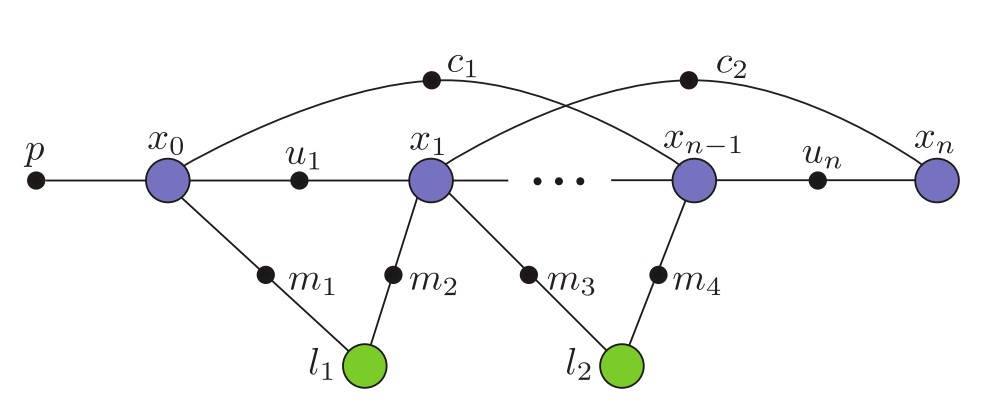
\includegraphics[width=.8\textwidth]{figs/isam_factor_graph.png}
    \caption{因子图示例\citep{kaess2012isam2}:紫色节点代表位姿状态,绿色节点代表三维点状态,黑色节点代表状态之间的约束因子。}
    \label{fig:isam_factor_graph}
\end{figure}

图\ref{fig:isam_factor_graph}展示了一类常见的因子图结构。按照图示的例子,一个SLAM问题中可能存在的约束有状态变量的先验约束$p$,相邻状态之间的相对位姿约束$u_1 \dots u_n$,非相邻状态之间的回路闭合约束$c_1,c_2$以及视觉观测约束$m_1 \dots m_4$等。而求解完整集束优化的过程就相当于最大化整个因子图中的所有约束的集合$\mathcal{Z}$关于所有状态集合$\mathcal{X}$的联合条件概率:
\begin{equation}
    P(\mathcal{Z}|\mathcal{X}) = \prod_{f_i\in\mathcal{Z}} P(f_i(\mathcal{X}_i))
\end{equation}
其中$\mathcal{X}_i$代表所有与约束节点$f_i$相邻的状态节点。通常会假设这是一个高度非线性系统,并且所有的约束$f_i$的噪声服从高斯分布$f_i\sim\mathcal{N}(\mu_i, \sigma_i^2)$。这样的的概率最大化问题通常被转化为非线性最小二乘(Non-linear Least Squares,NLS)问题来求解:
\begin{equation}
\begin{aligned}
    \mathcal{X}^\star &= \mathop{\arg\max}_{\mathcal{X}}
                         \prod_{f_i\in\mathcal{Z}} P(f_i(\mathcal{X}_i)) \\
                      &= \mathop{\arg\min}_{\mathcal{X}}
                         \sum_{f_i\in\mathcal{Z}} \frac{1}{2}
                         \lVert f_i(\mathcal{X}_i)) \rVert_{\sigma_i^2}^2
\end{aligned}
\end{equation}

\subsection{非线性最小二乘}

非线性最小二乘问题难以被直接求解,通常要使用迭代求解的方法来逼近局部最优解。如果变量的初值在全局最优解的附近,则一般可以使用牛顿法(Newton's method)迭代求解。如下给出了而一个典型的非线性最小二乘问题的形式:
\begin{equation}
\begin{aligned}
    \bm{x}^\star &= \mathop{\arg\min}_{\bm{x}} F(\bm{x}) \\
                 &= \mathop{\arg\min}_{\bm{x}}
                    \frac{1}{2} \Vert \mathbf{f}(\bm{x}) \Vert^2
\end{aligned}\label{eq:nlls}
\end{equation}
其中变量$\bm{x}\in\mathbb{R}$,$\mathbf{f}(\cdot)$为关于变量$\bm{x}$的非线性函数,即目标函数。

在局部最优解附近,最小化能量函数$F(\cdot)$等同于求解其梯度函数$\bm{g}(\cdot)$的零点(对于线性的函数则为唯一的零点),即:
\begin{equation}
    \bm{g} \doteq \nabla F = \begin{bmatrix}
        \frac{\partial F}{\partial x_1} &
        \frac{\partial F}{\partial x_2} &
        \cdots &
        \frac{\partial F}{\partial x_n}
    \end{bmatrix}^\top = \bm{0}
\end{equation}

采用牛顿法求解上述零点问题,记梯度函数$\bm{g}(\cdot)$的一阶导数为海森矩阵(Hessian matrix):
\begin{equation}
    \mathrm{H} \doteq \begin{bmatrix}
        \frac{\partial^2 F}{\partial x_1^2} &
        \frac{\partial^2 F}{\partial x_1 \partial x_2} &
        \cdots & \cdots &
        \frac{\partial^2 F}{\partial x_1 \partial x_n} \\
        %
        \frac{\partial^2 F}{\partial x_2 \partial x_1} &
        \frac{\partial^2 F}{\partial x_2^2} &
        & &
        \frac{\partial^2 F}{\partial x_2 \partial x_n} \\
        %
        \vdots & & \ddots & & \vdots \\
        \vdots & & & \ddots & \vdots \\
        %
        \frac{\partial^2 F}{\partial x_n \partial x_1} &
        \frac{\partial^2 F}{\partial x_n \partial x_2} &
        \cdots & \cdots &
        \frac{\partial^2 F}{\partial x_n^2}
    \end{bmatrix}
\end{equation}
求解如下线性系统:
\begin{equation}
    \bm{x} = -\mathrm{H} \enspace\setminus\enspace \bm{g}
    \label{eq:linsys}
\end{equation}

线性的问题中,当矩阵$\mathrm{H}$为正定矩阵时, 给定任意初值$\bm{x}$(这里选择了初值为$\bm{0}$)只需一步就可解得式\eqref{eq:nlls}的全局最优解。而对于非线性的情况,则需要多次迭代才能解得局部最优解。

\subsection{高斯-牛顿法}\label{sec:gn}

对于非线性最小二乘问题,牛顿法中计算函数$F(\cdot)$的准确海森矩阵$\mathrm{H}$的代价往往很大,甚至没有闭解。一些算法会寻求使用近似方法计算每次迭代的海森矩阵,比如拟牛顿法\citep{tingleff2004methods}(Qausi-Newton method)。拟牛顿法适用于一般的最小化问题,而对于非线性最小二乘问题,通常可以高斯-牛顿法(Gauss-Newton method)求解。高斯-牛顿法是用于求解非线性最小二乘问题的经典迭代算法,也是众多其他迭代算法的基础。

依然考虑非线性最小二乘问题\eqref{eq:nlls},使用高斯-牛顿法迭代求解,首先要给定变量的初值$\bm{x}=\bm{x}_0$。对其在当前点处进行泰勒展开,并忽略高阶项,可得目标函数$\mathbf{f}(\cdot)$在$\bm{x}_0$处的线性近似:
\begin{equation}
    \mathbf{f}(\bm{x}_0+\bm{\delta}) \simeq \mathbf{f}_0 + \mathrm{J}\bm{\delta}
\end{equation}
其中$\mathrm{J}\in\mathbb{R}^{m \times n}$是目标函数$\mathbf{f}(\cdot)$在$\bm{x}_0$处的雅各比矩阵(Jacobian)。式\eqref{eq:nlls}被转化为局部$\bm{x}_0$处的线性最小二乘子问题
\begin{equation}
    \bm{\delta}_{gn} =
        \min_{\bm{\delta}} \frac{1}{2}
        \Vert \mathbf{f}_0 + \mathrm{J}\bm{\delta} \Vert^2
    \label{eq:lls}
\end{equation}
使用牛顿法求解这个线性最小二乘子问题,构建正规方程(normal equation)并求解,可得高斯-牛顿法一次迭代的结果:
\begin{equation}
    \bm{\delta}_{gn} =
        -\left( \mathrm{J}^\top\mathrm{J} \right)
        \enspace\setminus\enspace
        \left( \mathrm{J}^\top\mathbf{f}_0 \right)
    \label{eq:normal_eq}
\end{equation}
将此结果更新至变量:$\bm{x}\leftarrow\bm{x}_0+\bm{\delta}$,然后不断重复以上过程,直至结果收敛。

式\eqref{eq:normal_eq}和\eqref{eq:linsys}的形式类似,也可以认为高斯-牛顿法和牛顿法的最大区别就是高斯-牛顿法使用了$\mathrm{J}^\top\mathrm{J}$来近似海森矩阵$\mathrm{H}$。

\subsection{信赖域方法}

除了高斯-牛顿法之外,还有一种经典的求解非线性最小二乘优化的算法:莱文贝格-马夸特(Levenberg-Marquardt,LM)法。它也被认为是带有阻尼因子的高斯-牛顿法,也是信赖域方法(trust region method)的前身\citep{jorge2006numerical}。

众所周知,一般的VO算法中,尺度是不可观测的(unobservable)——在VO的状态估计中,对全局所有的三维点坐标和相机位置进行统一的缩放,不会引起重投影误差的改变(在不考虑数值误差的情况下)。从求解VO集束优化问题的角度来看,这一性质造成了在直接使用高斯-牛顿法时海森矩阵的秩亏现象,即矩阵$\mathrm{J}^\top\mathrm{J}$为半正定的情况。此时直接使用矩阵分解求逆的方法求解线性最小二乘子问题就会得到数值不稳定的结果,比如解得的步长在某个方向过大等。

\subsubsection*{莱文贝格方法}

针对这一情况,莱文贝格在基础的高斯-牛顿法中引入了对迭代步长的直接约束,将原先每次迭代的线性最小二乘子问题改写为:
\begin{equation}
    \bm{\delta}_{l} =
        \mathop{\min}_{\bm{\delta}} \frac{1}{2}
        \left(
            \Vert \mathbf{f}_0 + \mathrm{J}\bm{\delta} \Vert^2 +
            \mu \Vert \bm{\delta} \Vert^2
        \right), \quad \mu > 0
\end{equation}
这样一来,原先高斯-牛顿法求解的正规方程就变成了
\begin{equation}
    \bm{\delta}_l =
        -\left( \mathrm{J}^\top\mathrm{J}+\mu\mathrm{I} \right)
        \enspace\setminus\enspace
        \left( \mathrm{J}^\top\mathbf{f}_0 \right)
    \label{eq:levenberg}
\end{equation}
其中的$\mu$就是所谓的阻尼因子(damping factor)。

阻尼因子控制住了每次迭代计算的步长的模。通常阻尼因子$\mu$具备下面三个性质\citep{tingleff2004methods}:
\begin{enumerate}
    \item 对于任意的$\mu>0$,海森矩阵$(\mathrm{J}^\top\mathrm{J}+\mu\mathrm{I})$正定,这一点保证了求得的步长$\bm{\delta}$处于能量下降的方向;
    \item 当$\mu\to\infty$时,求得的步长$\bm{\delta}$接近于梯度下降方向$-\frac{1}{\mu}\mathrm{J}^\top\mathbf{f}(\bm{x})$,当当前的变量$\bm{x}$ 的值距离最优解较远时,梯度下降的方向更容易符合预期;
    \item 当$\mu\to0$时,则求得的步长$\bm{\delta}$更接近于高斯-牛顿法的结果,如果当前变量$\bm{x}$的值较为接近最优解,则这样的步长更容易符合预期,因为在收敛点附近,真实的海森矩阵更接近标准的二次型形式。
\end{enumerate}
同时,由于正则项$\mu\mathrm{I}$的加入,修改后的海森矩阵$(\mathrm{J}^\top\mathrm{J}+\mu\mathrm{I})$一定为正定二次型矩阵,提升了求解的数值稳定性。

\subsubsection*{莱文贝格-马夸特方法}

莱文贝格在海森矩阵的每一个主元上都施加了同样的阻尼限制$\mu$,某种程度上将是对步长$\bm{\delta}$在各个梯度方向上施加了相同的限制,这显然不是最合理的做法。当$\mu$非常大的时候,一定程度上由原始海森矩阵$\mathrm{J}^\top\mathrm{J}$提供的信息就被抑制了,难以被利用。马夸特在莱文贝格的方法上进行了改进,根据海森矩阵的主元大小,对步长的不同梯度方向施加不同的阻尼:
\begin{equation}
    \bm{\delta}_{lm} =
        -\left( \mathrm{J}^\top\mathrm{J}+\mu\mathbf{diag}(\mathrm{J}^\top\mathrm{J}) \right)
        \enspace\setminus\enspace
        \left( \mathrm{J}^\top \mathbf{f}_0 \right)
\end{equation}
这样一来,在梯度较小的方向阻尼较小,$\bm{\delta}_{lm}$的分量也就较大,反之则阻尼较大,$\bm{\delta}_{lm}$的分量较小。得益于更合理的阻尼设置,相对于单纯的莱文贝格法,莱文贝格-马夸特方法在实际应用中的收敛效率要更好。

\subsubsection*{狗腿法}

狗腿法(Dog-Leg,DL)是另一个经典的求解非线性最小二乘优化的算法,也是信赖域方法的代表。莱文贝格-马夸特方法通过阻尼因子来间接地控制每一次迭代的步长,而狗腿法则显式地使用了信赖域来约束每一次迭代的步长。下面给出传统的使用狗腿法求解问题\eqref{eq:nlls}的步骤\citep{tingleff2004methods}。首先按照常规的求解步骤进行线性化,得到线性最小二乘子问题\eqref{eq:lls}。狗腿法首先使用高斯-牛顿法求解一个二阶迭代步
\begin{equation}
    \bm{\delta}_{gn} =
        -\left( \mathrm{J}^\top\mathrm{J} \right)
        \enspace\setminus\enspace
        \left( \mathrm{J}^\top \mathbf{f}_0 \right)
\end{equation}
然后使用最速下降法求解一个一阶的迭代步
\begin{equation}
    \bm{\delta}_{sd} =
        \frac{\lVert\bm{g}\rVert^2}{\lVert\mathrm{J}\bm{g}\rVert^2}
        \left( \mathrm{J}^\top \mathbf{f}_0 \right)
\end{equation}

狗腿法根据当前的信赖域半径$\Delta$和以上求解的两个步长来计算综合的迭代步$\bm{\delta}_{dl}$,当$\Delta$较大时,狗腿法倾向于选择高斯-牛顿法的迭代步$\bm{\delta}_{gn}$;当$\Delta$较小时则倾向于选择最速下降法的迭代步$\bm{\Delta}_{sd}$。

\subsection{鲁棒估计方法}

For least squares problems where the minimization may encounter input terms that contain outliers, that is, completely bogus measurements, it is important to use a robust function that reduces their influence\citep{ceres-solver}.

An unconstrained robustified nonlinear least squares (RNLLS) problem modifies the basic NLLS \eqref{eq:nlls}

\begin{equation}\label{eq:rnlls}
\begin{aligned}
    \bm{x}^\star &= \mathop{\arg\min}_{\bm{x}} G(\bm{x}) \\
                 &= \mathop{\arg\min}_{\bm{x}}
                    \frac{1}{2} \rho
                    \left( \lVert \mathbf{f}(\bm{x}) \rVert^2 \right)
\end{aligned}
\end{equation}

where the scalar function $\rho(\cdot)$ reweights the normal equation. Like solving the NLLS problems, we solve the RNLLS by finding the zero of the robustified gradient

\begin{equation}
    \bm{g} \doteq \nabla G = \rho' \mathrm{J}^\top \mathbf{f}(\bm{x})
\end{equation}

Note that $\rho'(\cdot)$ is also function of $\bm{x}$ (the dependence of $\mathrm{J}$ on $\bm{x}$ is ignored since $\mathbf{f}(\cdot)$ is assumed to be linear at current iteration $\mathbf{f}(\bm{x} + \bm{\delta}) \simeq \mathbf{f}(\bm{x}) + \mathrm{J}\bm{\delta}$), so the Hessian of $\bm{g}$ is

\begin{equation}
\begin{aligned}
    \mathrm{H}
           &=
              \rho' \mathrm{J}^\top \mathrm{J} +
              \frac{\partial\rho'(\bm{x})}{\partial\bm{x}}
              \mathbf{f}^\top(\bm{x})\mathrm{J} \\
           &=
              \rho' \mathrm{J}^\top \mathrm{J} +
              \frac{\partial\rho'}{\partial\lVert\mathbf{f}(\bm{x})\rVert^2}
              \frac{\partial\lVert\mathbf{f}(\bm{x})\rVert^2}{\partial\bm{x}}
              \mathbf{f}^\top(\bm{x}) \mathrm{J} \\
           &=
              \rho' \mathrm{J}^\top \mathrm{J} + \rho''
              \frac{\partial\lVert\mathbf{f}(\bm{x})\rVert^2}{\partial\bm{x}}
              \mathbf{f}^\top(\bm{x}) \mathrm{J} \\
           &\simeq
              \rho' \mathrm{J}^\top \mathrm{J} + 2\rho''
              \mathrm{J}^\top \mathbf{f}(\bm{x}) \mathbf{f}^\top(\bm{x}) \mathrm{J} \\
           &=
              \mathrm{J}^\top \left(
                  \rho'\mathrm{I} + 2\rho''
                  \mathbf{f}(\bm{x}) \mathbf{f}^\top(\bm{x})
              \right) \mathrm{J}
\end{aligned}
\end{equation}

The robustified normal equation is given by

\begin{equation}
    \mathrm{J}^\top \left(
        \rho'\mathrm{I} + 2\rho''
        \mathbf{f}(\bm{x}) \mathbf{f}^\top(\bm{x})
    \right) \mathrm{J} \bm{\delta}
    =
    -\rho' \mathrm{J}^\top \mathbf{f}(\bm{x})
\end{equation}
     % section : 基于非线性优化方法的状态估计

\section{SLAM状态估计相关工作}

VSLAM和VISLAM都需要根据系统的先验估计、传感器观测来对系统的状态进行估计,可能包括实时的位姿状态、传感器状态、场景三维点状态以及其他可能的信息。主流的SLAM方法根据状态估计的方法可以分为基于扩展卡尔曼滤波(Extended Kalman Filter,以下简称EKF)的滤波法和基于非线性最小二乘(Nonlinear Least Squares)的优化法。两类方法没有本质上的区别,都是使用最大化后验概率(Maximum A-Posteriori estimation,以下简称MAP)的思想求解非线性系统的最优状态估计,但是在求解的速度、精度以及算法的可扩展性上存在一定差异。根据对视觉信息的利用方法又可以分为直接法(direct methods)和特征法(feature-based methods)。使用关键点进行图像匹配,并使用重投影误差(reprojection error)作为视觉约束求解三维结构的方法称为特征法。直接使用稠密或稀疏的图像像素信息,并使用光度误差(photometric error)作为视觉约束的方法称为直接法。

\subsection{基于滤波法的SLAM状态估计}

一般来讲滤波法的时间复杂度小于同规模的优化法,早期由于计算能力的限制,选择滤波法进行状态估计是一种合理的选择。MonoSLAM\citep{davison2007monoslam}是最早的单目VSLAM系统之一。MonoSLAM使用了EKF求解相机状态和三维点状态,也是最早的滤波法VSLAM系统之一。在状态估计阶段,MonoSLAM快速地将旧的相机状态通过边缘化操作消去,将系统的状态数量限制在$O(N)$,其中$N$为三维点的数量,同时状态估计的时间复杂度被限制在了$O(N^3)$。因此MonoSLAM的运行时间得到了限制,不至于随着时间无限增长。但由于MonoSLAM过早地将相机状态进行边缘化,一部分尚未收敛的相机状态就将错误的信息留在了系统的状态中,导致了较大的误差累积。另一方面,频繁的边缘化操作也就导致了系统状态的协方差矩阵变得稠密,无法利用稀疏的求解方法进行加速,这一点也是基于EKF的算法的通病。

另一个经典的基于EKF的SLAM系统是MSCKF\citep{mourikis2007multi}。MSCKF全称是多状态约束卡尔曼滤波(Multi-State Constraints Kalman Filter)。与MonoSLAM不同的是,MSCKF使用了相机状态窗口的概念,计算大小为$M$的系统的EKF更新,其中$M$为状态窗口的大小。因此MSCKF将状态估计的实现复杂度限制在了$O(M^3)$。由于在SLAM问题中,三维点的数量往往远远大于相机状态的数量:$N \gg M$,MSCKF算法可以达到实时性的要求,效率要高于MonoSLAM。又由于MSCKF保留了一定数量的历史相机状态,而不是尽早地将旧的状态消去,因此误差累积更小,更适合长时间、大尺度的应用。

此外,MSCKF还使用了IMU信息,因此属于VISLAM。MSCKF使用了一般的迭代式IMU积分技术,即直接通过对IMU读数进行积分,得到最新相机状态的先验分布,而将图像特征信息作为观测,经过EKF更新融合视觉信息和IMU信息。MSCKF的算法的框架如下:
\begin{enumerate}
    \item 状态传播:对于IMU读数,使用龙格库塔法对其进行积分,同时根据IMU噪声参数更新状态的先验协方差矩阵;
    \item 图像注册:每当得到新的图像时,根据当前的最新状态以及IMU-相机外参对状态进行增广,得到状态的先验。并对图像进行处理,提取视觉特征,更新特征跟踪信息等;
    \item 状态更新:选择合适的时机,通过EKF更新融合视觉信息和IMU信息,得到后验状态分布。
\end{enumerate}

MSCKF的状态窗口包括最新的相机状态和保留在窗口内的部分历史相机状态。在$k$时刻其状态变量定义如下:
\begin{equation}
    \bm{X}_k \doteq
    \left[
        \bm{X}_{\textrm{IMU}_k},
        \prescript{G}{}{\mathrm R}_{C_1},
        \prescript{G}{}{\bm p}_{C_1},
        \cdots,
        \prescript{G}{}{\mathrm R}_{C_N},
        \prescript{G}{}{\bm p}_{C_N}
    \right]
\end{equation}
除了MSCKF,后续的一些主流的VISLAM也大多使用了如上的相机-IMU状态定义。

如前面描述的,MSCKF算法是无三维结构信息的,也就是只保留相机状态,而不估计三维点的状态。在状态估计前选取一部分视觉特征,快速地通过三角化计算出对应的三维点状态,然后快速地通过边缘化操作消去,最后再对相机状态进行更新。MSCKF依据一定的策略来选取特征,以下两条规则会触发状态更新:
\begin{enumerate}
    \item 这种情况触发得最频繁:当一个视觉特征在被连续跟踪数帧后丢失(移出相机视野)时会触发一次状态更新。这种情况下,由于在最新的相机中特征已经丢失,因此后续它不会再更新,可以通过边缘化操作将它消去。
    \item 每次得到图像时,MSCKF都会增广当前的状态。为了尽可能保留长的基线和几何信息,当相机状态数量达到上限$M_{max}$时,MSCKF选择从状态中第二旧的相机开始,平均地选择$M_{max}/3$个相机状态。使用被选中的相机观测到的特征跟踪来进行EKF更新,最后消去对应的状态。
\end{enumerate}

MSCKF求解的状态估计仍然不是全局最优的。前面提到,被消去的状态的信息要先以边缘化的方式将保留下来,即得到剩余状态的边缘概率分布。一部分剩余状态的雅各比矩阵,其线性化点的被永远固定在了发生边缘化的时刻。后续即使状态值发生了改变,旧的雅各比矩阵由于已经被编码进了先验状态分布中而不能再改变,而随后得到的新的观测信息总是会根据最新的状态值计算雅各比矩阵,这就造成了所谓的信息不一致(inconsistency)。客观上,信息不一致造成了MSCKF的状态估计在某些不可观测的自由度上引入了一些不必要的误差。为了解决信息一致性的问题,后续版本的MSCKF2.0\citep{li2012improving}引入了FEJ技术(First Estimate Jacobian)技术\citep{huang2008analysis},在计算新的观测关于旧的变量的雅各比矩阵时,总是使用状态边缘化发生时刻的线性化点,一定程度上缓解了这个问题,提高了精度。另一些侧重于解决信息不一致性的SLAM相关工作有\citep{huang2011observability}和\citep{huang2013quadratic},通过选用特殊的线性化点的方式保持了系统的不可观测的自由度,以及使用了一个变种EKF算法弥补错误不可观测自由度的\citep{barrau2015ekf},也可以提高状态估计的精度。

\subsection{基于集束调整优化的SLAM状态估计}

随着硬件能力的发展,状态优化的计算效率已经越来越不再是SLAM系统的瓶颈所在。一方面,由于优化法和滤波法并没有时间复杂度上的差异,也有许多算法能够利用SLAM问题的稀疏性和局部性减少优化的计算量,比如使用舒尔补、稀疏矩阵分解甚至增量式优化的方法。一些高效的基于优化法的SLAM系统已经能在效率上逼近甚至超越基于滤波法的SLAM系统。另一方面,优化法在精度上相对于滤波法有着不可比拟的优势。尽管有很多的手段提升滤波法的精度,但是由于难以求解全局最优解,滤波法仍然会有较大的误差累积。前面提到,滤波法和优化法在概率上都是MAP估计,由于每次求解状态估计,EKF都只做一次线性化并进行一次更新,而优化法则通过迭代不断更新线性化点求解直至收敛,因此滤波法可以认为是使用了一轮迭代的优化法。显而易见,相比于优化法,滤波法虽然速度更快,但不保证状态收敛。而且基于优化法的SLAM可以在基础的视觉观测约束、IMU约束上其他约束,进一步消除误差累积,基于滤波法的SLAM则在这方面的可扩展性上稍差。因此,越来越多的主流SLAM系统已经在使用基于优化法的状态估计。

PTAM\citep{klein2007parallel}是最经典的基于优化法的VSLAM系统的代表。在系统架构上,PTAM创新性地将局部的相机跟踪定位和全局优化分发到两个线程中运行。在前端相机跟踪线程中,PTAM对系统的移动速度进行了建模,使用估计的速度预测相机的位姿。借助于预测的位姿,可以得到旧的视觉特征点在新的相机图像中的投影,从而缩小特征匹配时的搜索范围。给定特征匹配,通过最小化重投影误差可以得到相机位姿的粗略估计。由于前端线程只求解位姿,这一步可以实时运行。当前端线程还会筛选出质量较高的图像帧作为关键帧(keyframe)加入到后端全局优化线程中。而在后端全局优化线程中,PTAM使用了集束调整来求解全局的地图。全局地图的求解时间会随关键帧的增长而呈$O(M^3)$级别的增长,受限与此,PTAM将关键帧的数量限制在了$100$帧。但即便如此,将相机跟踪和全局优化分发到不同的线程中执行的思想被证明可以大幅提高基于优化法的SLAM的性能,在随后的SLAM研究工作中,这种思想被大量借鉴。目前的主流SLAM系统大多数都使用了多线程的方法提高系统的效率。

ORB-SLAM\citep{mur2015orb,murorb2}是另一个经典的VLSAM工作,也是目前最先进的SLAM系统之一。ORB-SLAM使用了ORB特征来提升跟踪质量。在PTAM的基础上,ORB-SLAM还额外利用了全局地图的信息,加入了重定位和和回路闭合模块。同样的,ORB也使用了多线程架构:局部相机跟踪、地图优化和回路闭合被分发到三个不同的线程中执行。局部相机跟踪线程维护了一个由关键帧组成的滑动窗口,会适时地优化最新关键帧和与其具有共视关系的一系列关键帧。由于局部窗口大小固定,局部跟踪线程的计算时间被限制在一个可接受的水平。为了尽量避免全局优化,在回路闭合线程中,ORB-SLAM使用了最小生成树建立的Essential Graph的方法来构建关键帧之间的回路约束。回路闭合的过程中也没有包括三维点状态的求解,Essential Graph以较低的计算开销获取了较好的回路闭合性能。

OKVIS\citep{leutenegger2015keyframe}是另一个基于优化法的SLAM系统。同时还是VISLAM的经典框架之一。与ORB-SLAM不同的是,OKVIS仅维护了一个局部的滑动窗口优化。由于不包含全局地图优化,OKVIS并不具备回路闭合和重定位能力。OKVIS在相机跟踪部分使用了和MSCKF类似的迭代式IMU积分技术,随后通过滑动窗口优化,同时最小化IMU运动误差和重投影误差,得到包含比较准确的尺度信息的状态估计结果。同时,OKVIS在保持优化的稀疏性的前提下使用了包含边缘化的滑动窗口优化,以提升优化的精度。滑动窗口会随着时间增长逐渐滑动,滑出窗口的状态一般需要进行边缘化,为了尽可能保持优化的稀疏性,OKVIS会根据滑出窗口的是否为关键帧来判断是否要进行完整的边缘化操作。

VINS-Mono\citep{qin2018vins}则是最新的一个较为完整的VISLAM系统实现。相对于以上的SLAM系统,VINS-Mono的框架更为完整,包含了鲁棒的初始化模块、包含边缘化的滑动窗口优化模块、重定位模块和全局优化模块。同样,这些模块被分发到了不同的线程中执行,以提升效率。

VINS-Mono使用了一个松耦合的方式对系统的状态进行初始化。在初始化阶段,VINS-Mono使用视觉SfM方法由一系列初始帧构建一个小规模的地图,然后通过与独立的IMU积分算法构建的初始位姿进行对齐,获取初始的地图状态和位姿状态,以及一系列初始的IMU状态参数。在滑动窗口模块,VINS-Mono首先通过KLT跟踪获取每一帧的初始位姿估计。在优化部分,VINS-Mono借鉴了OKVIS的做法,使用稀疏求解器求解状态估计,同时使用了类似OKVIS的选择性边缘化策略来保持优化的稀疏性。不同的是,VINS-Mono使用了的基于IMU预积分\citep{davison2007monoslam}技术,而不是传统的迭代式IMU积分,以提升IMU状态的优化效果。对于滑出窗口的状态,如果判断为关键帧,则会被加入到后端的全局优化中。全局优化运行于独立的线程,VINS-Mono使用了位姿图优化的方式对这些历史关键帧进行进一步更新,提供给回路闭合模块使用。VINS-Mono在系统的功能、速度和精度上达到了较高的水准。而且其移动端的版本VINS-Mobile\citep{li2017monocular}经过精简,可以在移动设备上达到实时的性能。

\subsection{基于直接法的SLAM系统状态估计}

以上介绍的SLAM系统均基于特征法。另一类直接法SLAM系统近年来也获得了较大的关注。特征法和直接法也没有绝对的优劣之分,特征法利用了图像中的关键信息,因此通常对于几何误差(如相机内参的误差)和图像噪声(如光照变化、卷帘快门相机的图像撕裂)更为鲁棒,但是关键点的提取和匹配通常比较耗时;直接法不需要提取和匹配关键点,因此速度较快,但对图像噪声较为敏感;另一方面,由于直接法通常利用了更多图像信息,因此在弱纹理情况下表现更好,而且其构建的地图往往比较稠密,可以进一步提供给三维重建算法使用。

DSO(Direct Sparse Odometry)\citep{engel2018direct}是目前最先进的直接法VSLAM系统之一。DSO使用了类似\citep{jin2003semi}提出的稀疏直接法进行跟踪,这一点与以往的大部分直接法VSLAM都不同。DSO也使用了优化法进行状态估计。除了传统直接法中使用的光度误差,DSO还对场景中的光照进行建模,提出了使用曝光时间、镜头晕影(lens vignetting)和非线性相应函数。这一改进使得DSO在光照变化的场景下具有更好的精度和鲁棒性。

类似OKVIS,DSO也使用了包含边缘化的滑动窗口优化方法。为了保证滑动窗口中的相机状态在三维空间中有较好的分布,DSO设计了一个特殊设计的评分函数对关键帧进行评分。当状态数量达到上限时,DSO会根据评分挑选需要消去的相机状态。为了保持稀疏性,DSO也会有选择地对消去的状态进行边缘化。

\subsection{增量式集束调整方法}

在实现SLAM算法时,需要在算法的精度和性能两者中做出权衡。完整的集束调整包括了对所有历史状态的所有观测,虽然可以获得最优的状态估计,但其计算代价往往是难以接受的。在一些对性能要求高的应用场景,例如AR应用和自动驾驶应用中,算法的性能往往决定了它的可用性甚至安全性。随着这类应用对实时的、高效SLAM算法需求的日益增加,一些致力于在保证一定精度的前提下降低计算代价的集束调整算法应运而生,其主要通过两种策略来减少算法的计算量。一类是针对应用场景的特点减小集束调整问题的规模,基于前几节的介绍,可以总结出以下几种方式:
\begin{itemize}
    \item 全局优化的规模:只保留状态变量,而不保留三维点变量,如ORB-SLAM的Essential Graph和VINS-Mono的位姿图优化;
    \item 基于历史状态窗口:只估计最近的数个历史状态或一系列选定的数个历史状态,OKVIS、VINS-Mono等的滑动窗口优化;
    \item 基于关键帧:只估计一部分选定的携带了足够信息的历史状态,而放弃一些冗余历史状态,如OKVIS、VINS-Mono等。
\end{itemize}
以上的方法通常也可以结合,或搭配多线程技术使用。

另一种策略是通过深入分析集束调整问题的特点,做针对性优化,减少冗余的计算。集束调整问题通常具有非常特殊的性质,合理利用这些性质,可以帮助更高效地求解SLAM系统的状态估计。比如,在SLAM系统中,通常需要求解的三维点变量的数量要远大于状态变量的数量,而且通常状态约束集中在状态与状态之间、状态与三维点之间,而一般不会直接出现在三维点与三维点之间。这就导致集束调整构建的正规方程具有特别的稀疏结构,如图~\ref{fig:sparse_matrix}。应该利用这种稀疏结构,并且在优化的过程中尽可能保持这种稀疏性。另外,在线的集束调整中,通常只有较新加入的变量会发生比较大的变动,旧的变量由于经过持续的优化而变动很小。可以利用这种局部的性质,只对少部分变量进行更新,从而减少集束调整的计算量。

以iSAM系列(主要包括iSAM\citep{kaess2008isam}和iSAM2\citep{kaess2012isam2})为例,增量式集束调整算法很好地利用了SLAM集束调整问题的稀疏性和局部性,实现了高效的求解。iSAM系列的工作主要深入分析了优化求解的以下几条特点:
\begin{itemize}
    \item 对观测的雅各比矩阵进行QR分解,或者对信息矩阵进行Cholesky分解得到平方根信息矩阵(square root information matrix)的过程,等同于使用消元法将因子图转化成贝叶斯网络的过程;
    \item 矩阵分解时产生的填充现象(fill-in),则等同于因子图转化过程中,多出来的变量之间的边;
    \item 同样,在矩阵分解时,选定不同的主元顺序(pivoting)对应于因子图转化过程中变量的消去顺序,其所产生的填充现象的程度也是不同的,如图~\ref{fig:fill_in}。
\end{itemize}

\begin{figure}[htb!]
    \centering
    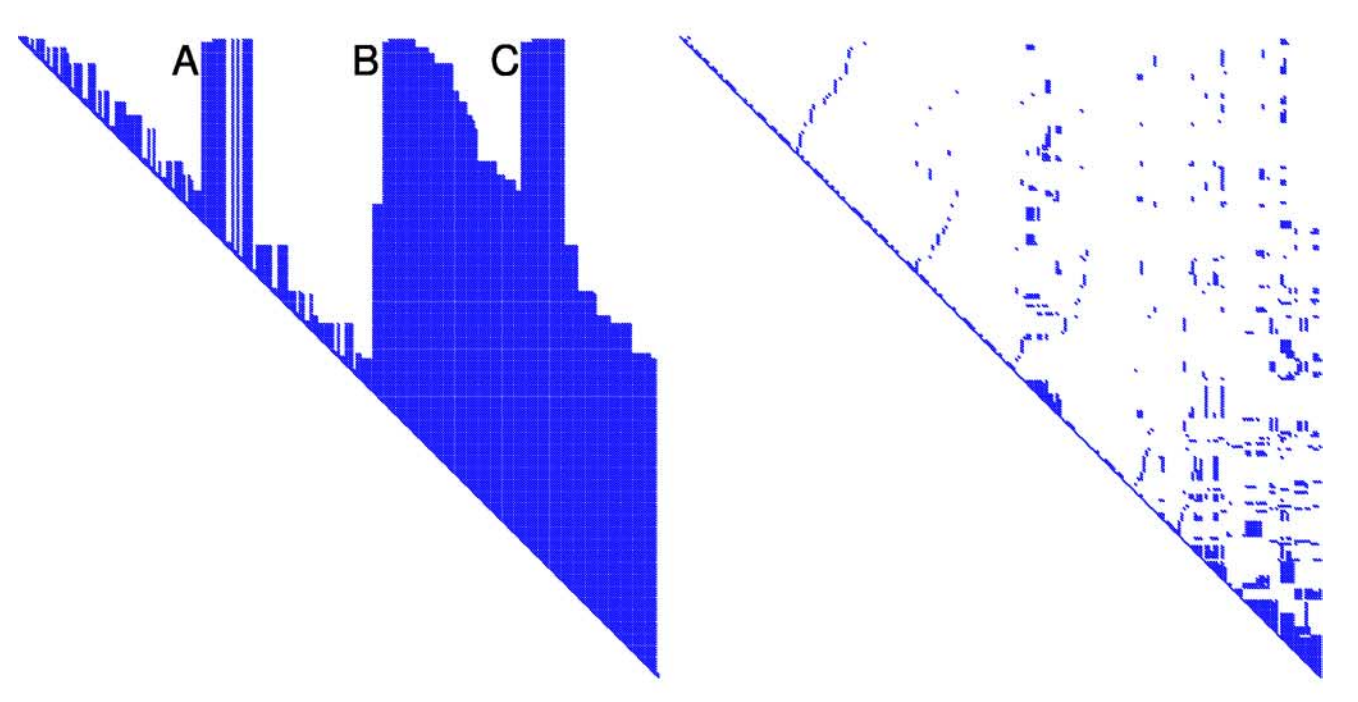
\includegraphics[width=.8\textwidth]{Pictures/sparse_pattern.png}
    \setcitestyle{sort&compress,longnamesfirst,square,numbers}
    \caption{信息矩阵稀疏结构\citep{kaess2008isam}:左图代表按照一般的消元顺序得到的平方根信息矩阵,右图代表先使用COLAMD算法选择一个较优的消元顺序,然后得到的平方根信息矩阵。可见,变量消去顺序对矩阵分解产生的填充现象有巨大影响。}
    \label{fig:fill_in}
\end{figure}

因此,完全可以用分析因子图的转化过程来代替直接对矩阵分解过程的分析。具体来说,iSAM系列算法使用一种特殊的贝叶斯树结构编码并维护了优化过程中分解得到的平方根信息矩阵,使得每次更新平方根信息矩阵时只要做很少的改动即可:
\begin{enumerate}
    \item 减少填充现象:通过一些启发式算法如COLAMD\citep{davis2004algorithm}、CHOLMOD\citep{chen2008algorithm}算法找到次优(suboptimal)的变量消去顺序,使得因子图转化为贝叶斯置信网络的过程中尽可能地不产生新的边;
    \item 使用贝叶斯树编码平方根信息矩阵:对于因子图转化而来的贝叶斯置信网络,使用特殊的贝叶斯树来编码其中的稀疏结构和变量因果关系;
    \item 即时重新线性化:利用贝叶斯树中的编码的变量因果关系,每当因子图中加入新的变量或约束,则即时地对影响到的变量进行线性化,避免每次都重新构造整个平方根信息矩阵;
    \item 局部变量更新策略:通过设置一个阈值$\epsilon$,在求解得到变量的增量$\Delta$后,根据其是否满足$|\Delta|>\epsilon$来判断是否需要更新这个变量。
\end{enumerate}

这样,维护一个增量求解的集束调整算法的时间复杂度就会远低于一般的完整的集束调整,从而在不损失精度或损失很少的精度情况下将SLAM算法的速度提升一个甚至数个数量级。
 % section : 视觉惯性SLAM相关工作

\section{本文内容及结构}

本章总结了VSLAM、VISLAM工作中关于状态估计的研究现状。对基于滤波方法和基于非线性优化方法的状态估计进行了解释。阐述了当前SLAM领域的常用的基于滤波法和基于集束调整优化的状态估计方法啊,列举并分析了这些SLAM系统中状态估计方法的优缺点,并简要介绍了目前最高效的增量式集束调整方法的思想。接下来本文将着重介绍一个面向VISLAM的通用集束调整框架的实现。第\ref{ch:vislam}章将详细介绍目前最新的基于IMU预积分约束的目标函数,阐述IMU传感器的基本模型和使用方法,以及如何将惯性辅助模块集成进传统VSLAM的集束优化框架。包括IMU预积分方法实现,IMU状态估计的方法;第\ref{ch:ba}章将详细介绍基于增量式集束调整的SLAM后端优化模块。包括增量式集束调整的原理和流程,以及工程实现上的细节,并分析与其他增量式算法之间的共性和优劣;第\ref{ch:exp}章通过实验结果评估求解效率,进一步验证本文提出的基于IMU预积分的增量式集束调整框架的效率和精度;第\ref{ch:con}章给出本文的结论以及后续工作的展望。
